\documentclass[
  digital, %% This option enables the default options for the
           %% digital version of a document. Replace with `printed`
           %% to enable the default options for the printed version
           %% of a document.
  twoside, %% This option enables double-sided typesetting. Use at
           %% least 120 g/m² paper to prevent show-through. Replace
           %% with `oneside` to use one-sided typesetting; use only
           %% if you don’t have access to a double-sided printer,
           %% or if one-sided typesetting is a formal requirement
           %% at your faculty.
  table,   %% This option causes the coloring of tables. Replace
           %% with `notable` to restore plain LaTeX tables.
  lof,     %% This option prints the List of Figures. Replace with
           %% `nolof` to hide the List of Figures.
  lot,     %% This option prints the List of Tables. Replace with
           %% `nolot` to hide the List of Tables.
  %% More options are listed in the user guide at
  %% <http://mirrors.ctan.org/macros/latex/contrib/fithesis/guide/mu/fi.pdf>.
]{fithesis3}
%% The following section sets up the locales used in the thesis.
\usepackage[resetfonts]{cmap} %% We need to load the T2A font encoding
\usepackage[T1,T2A]{fontenc}  %% to use the Cyrillic fonts with Russian texts.
\usepackage[
  main=english, %% By using `czech` or `slovak` as the main locale
                %% instead of `english`, you can typeset the thesis
                %% in either Czech or Slovak, respectively.
  english, german, russian, czech, slovak %% The additional keys allow
]{babel}
%% The following section sets up the metadata of the thesis.
\thesissetup{
    date          = \the\year/\the\month/\the\day,
    university    = mu,
    faculty       = fi,
    type          = bc,
    author        = Attila Zsíros,
    gender        = m,
    advisor       = Mgr. Jan Čejka,
    title         = {Using Kalman filters for pose estimation of mobile devices in simulated                     underwater environments},
    TeXtitle      = {Using Kalman filters for pose estimation of mobile devices in simulated                     underwater environments},
    keywords      = {Augmented reality, Extended Kalman filter, iMareCulture, Kalman filter,                     Motion tracking, Odometry, Pose estimation},
    TeXkeywords   = {Augmented reality, Kalman filter, Extended Kalman filter, iMareCulture,                     Motion tracking, Odometry, Pose estimation},
    abstract      = {This is the abstract of my thesis, which can

                     span multiple paragraphs.},
    thanks        = {These are the acknowledgements for my thesis, which can

                     span multiple paragraphs.},
    bib           = bibliography.bib,
}
\usepackage{makeidx}      %% The `makeidx` package contains
\makeindex                %% helper commands for index typesetting.
%% These additional packages are used within the document:
\usepackage{paralist} %% Compact list environments
\usepackage{amsmath}  %% Mathematics
\usepackage{amsthm}
\usepackage{amsfonts}
\usepackage{url}      %% Hyperlinks

\usepackage[textwidth=2.5cm]{todonotes}
\setlength{\marginparwidth}{2.5cm}

\usepackage{siunitx}

\usepackage{markdown} %% Lightweight markup
\usepackage{listings} %% Source code highlighting
\lstset{
  basicstyle      = \ttfamily,%
  identifierstyle = \color{black},%
  keywordstyle    = \color{blue},%
  keywordstyle    = {[2]\color{cyan}},%
  keywordstyle    = {[3]\color{olive}},%
  stringstyle     = \color{teal},%
  commentstyle    = \itshape\color{magenta}}
\usepackage{floatrow} %% Putting captions above tables
\floatsetup[table]{capposition=top}
\begin{document}
\renewcommand{\sectionautorefname}{Section}
\chapter*{Introduction}
    \addcontentsline{toc}{chapter}{Introduction}
    \section{Introduction}
    The seabed is often called the biggest museum in the world. Thousands of shipwrecks, ancient flooded cities, and other structures form our underwater cultural heritage. Because many of these objects are deprived of their context when exhibited on land, some sites offer \textit{in situ} experience, where scuba divers have the chance to experience them in their original surroundings \cite{unesco}. 

    Immersive technologies are extensively used at such archaeological sites since they can present information connected to user's location, e.g., historical facts, visual navigation, or even provide an augmented reality view of the original state of the structure. A European Union project, named iMareCulture\footnote{https://imareculture.eu/}, is concerned about developing such applications. One branch of the project, which this thesis is a part of, aims at implementing virtual visits in augmented reality.
    
    As Aron et al. defined \cite{inertial_video}: ``Augmented reality (AR) systems supplement the real world with virtual (computer-generated) objects that appear to coexist seamlessly in the same space as the real world.'' A difficult task in AR is tracking, i.e., the real-time pose recovery from monocular video streams. Among other tracking methods \cite{fusion01}, there are two major ones that the thesis is dealing with:
    
    \begin{itemize}
      \item Vision-based methods provide high accuracy but slow update rates and require line-of-sight between the camera and the markers;
      \item Inertial tracking, performed by the sensors from the inertial sensor unit (IMU), provides high-frequency measurements but is unreliable to track position for long periods of time due to problems with sensor bias and drift.
    \end{itemize}
    
    The goal of this thesis is the fusion of these two complementary approaches to get more accurate pose estimations than by using any of them alone. It extends an existing prototype of a vision-based AR application for Android phones and tablets. The application uses methods from ArUco library\footnote{ArUco is an OpenSource library for camera pose estimation using squared markers. \url{https://www.uco.es/investiga/grupos/ava/node/26}} with 2D barcode markers, detected by the camera, that are to be distributed in the archaeological site. For sensor fusion, a common data fusion algorithm that combines and smooths the measured values - the Kalman filter - is utilized.
    
    The first chapter discusses the available AR platforms with references to related works. The next two chapters introduce the theoretical background of the tracking methods, the relations between the coordinate frames, and the Kalman filtering.
    
    The fourth chapter is about experiments. Firstly, it presents the technical equipment and testing conditions. Secondly, it shows the Kalman filter performance from more straightforward cases (only a single marker with accelerometer) to the complex ones, when all IMU sensors along with multiple markers are involved. Successively, motion tracking is used as ground-truth, and several non-linear variants, such as the Extended and Unscented Kalman filter, are built and compared to each other.
    
    In the last chapter, an upgraded working prototype of the AR application is tested in the Underwater Archaeological Park of Baia in Italy. The quality of the prototype is discussed, and gives suggestions for future development.

\chapter{Abstract}
\section{English}
This thesis analyzes the effect of underwater conditions on a chosen pose estimation system that solves the task of determining the position and orientation of the device in its environment. Within the project iMareCulture, it contributes to the application of augmented reality in underwater museums.

First, a marker-based visual-inertial robotic pose tracking system that uses the extended Kalman filter (EKF) is utilized for the use with smartphone recordings. Second, the underwater environment is simulated in post-processing of the marker detection results by (1) discarding the detected markers according to their distance to simulate poor visibility, and (2) by corrupting the detected tag corners by artificial noise to simulate water turbidity. The simulations take place in a laboratory equipped with an external motion capture system as ground truth for evaluating the accuracy of the pose estimated by the utilized system.

The results show that the tracking accuracy does not significantly change with a decreasing number of detected markers. Thus, the markers can be placed more sparsely in the environment, or the system can discard redundant markers to reduce the computational cost. Furthermore, provided correct EKF settings, the system produces accurate pose estimates even with a high amount of noise corruption, simulating a very turbid environment.

\section{Slovak}

\chapter{Background}
    \begin{figure}
        \includegraphics[width=10cm]{img/Baia2.jpg}
        \caption{A tablet housed in a waterproof case showing an original reconstruction of Villa a Protiro.}
        \label{fig:baia2}
    \end{figure}

    The seabed is often called the biggest museum in the world. Throughout the history of human civilizations, entire cities have been flooded, and thousands of ships have sunken to the bottom of the lakes, seas, and oceans. In this subaqueous environment, they have been safely protected for thousands of years. Now they are a part of our cultural heritage in the same way as the heritage on land.
    
    Advances in technology have made the underwater world more accessible and therefore brought these sites within reach. The visitors are offered in situ experiences, which include dive trails, submersible tours for non-divers, and underwater museums \cite{unesco_online}.
    
    \textbf{Project iMare-Culture} focuses on promoting them to the wide public through the use of interactive technologies, virtual reality (VR), augmented reality (AR), and serious games\footnote{A serious game is a game designed for a primary purpose other than pure entertainment.}; all designed by scientists, researchers, archaeologists, and museum experts coming from eight Mediterranean countries.
    
    This thesis is a part of augmented reality research for this project. Figure \ref{fig:baia2} shows an example of AR usage, where the scuba diver is holding a tablet housed in a waterproof case, and observing an original reconstruction of Villa a Protiro in the Archaeological Underwater Park of Baia, Italy.

\chapter{Pose estimation for Augmented Reality}
As Azuma defined in 1997, AR systems supplement the real world with virtual (computer-generated) objects that appear to coexist seamlessly with the real world. Besides aligning real and virtual objects with each other, these systems have to be interactive and in real time \cite{97azuma}. In contrast with VR, where the user is immersed in a virtual environment, AR allows interaction with virtual objects in a seamless way.

The main AR research topics are Tracking Techniques, Interaction Techniques, Calibration and Registration, AR Applications, and Display Techniques \cite{17ISMAR}. The most popular amongst them are the tracking techniques, since good pose tracking is vital to deliver a seamless AR experience.

The tracking techniques are concerned with determining the pose of the camera, i.e., its position and orientation relative to a reference frame. Despite the enormous progress in this field in the last ten years, it is still challenging to achieve low latency tracking with high precision, accuracy, jitter, and lag in a mobile device. If we compare AR and VR again, but now in terms of tracking requirements, AR pose tracking is more demanding, since errors in registration are easier to detect by the user \cite{93Azuma}.

The tracking problem gets even more complex in underwater environments, where the system has to be waterproof, has to withstand the high pressure of diving depth, cannot rely on GPS, and the captured images suffer from turbidity effects caused by the medium.

Furthermore, the amount and cost of sensors packed in smartphones are much more limited than in specialized devices used in, for example, robotics \cite{vi-sensor}. As a consequence, the measurements are noisier and biased. Tracking techniques tackle these problems by integrating several sensors with complementary characteristics into a sensor fusion filter.

This chapter gives an overview of the popular pose estimation techniques and their utilization in the sea.

    \section{Visual tracking}
    Vision-based techniques use computer vision methods to calculate the camera pose relative to real-world objects \cite{99SoYou,02Pinz}. 
    
    They provide high accuracy over a large workspace, as well as low jitter and no drift. The frames are grabbed at rates of 30--60~Hz. 
    
    The general drawbacks include that they require line-of-sight between the camera and the detected target, and that motion blur in the image during drastic motions leads to temporary loss of real-time tracking abilities.  

        \subsection{Camera calibration}
        \todo[inline]{... When the image is rectified, the it can be used for marker detection. The targets of the detector are either markers (marker-based tracking) or distinctive features in the image (marker-less tracking). }
        
        \begin{figure}
        \begin{center}
            \begin{minipage}{.29\textwidth}
                \begin{center}
                    \includegraphics[width=.6\textwidth]{img/Markers/AprilTag.png} \\
                    \footnotesize(a) AprilTag \cite{AprilTag} \\
                    \vspace{0.6cm}
                    \includegraphics[width=.6\textwidth]{img/Markers/Elipses.png} \\
                    \footnotesize(d) Ellipse \cite{Ellipse} \\
                    \vspace{0.6cm}
                    \includegraphics[width=.6\textwidth]{img/Markers/reacTIV.png} \\
                    \footnotesize(d) reacTIVision \cite{reacTIVision} \\
                \end{center}
            \end{minipage}
            \begin{minipage}{.29\textwidth}
                \begin{center}
                    \includegraphics[width=.6\textwidth]{img/Markers/ARTag.jpg} \\
                    \footnotesize(b) ARTag \cite{ARTag} \\
                    \vspace{0.6cm}
                    \includegraphics[width=.6\textwidth]{img/Markers/CCTag.png} \\
                    \footnotesize(e) CCTag \cite{CCTag} \\
                    \vspace{0.6cm}
                    \includegraphics[width=.6\textwidth]{img/Markers/RUNE.png} \\
                    \footnotesize(e) RUNE-Tag \cite{RUNETag} \\
                \end{center}
            \end{minipage}
            \begin{minipage}{.29\textwidth}
                \begin{center}
                    \includegraphics[width=.6\textwidth]{img/Markers/ARToolKit.pdf} \\
                    \footnotesize(c) ARToolKit \cite{ARToolKit} \\
                    \vspace{0.6cm}
                    \includegraphics[width=.6\textwidth]{img/Markers/Intersense.png} \\
                    \footnotesize(e) Intersence \cite{Intersence} \\
                    \vspace{0.6cm}
                    \includegraphics[width=.6\textwidth]{img/Markers/FourierTag.png} \\
                    \footnotesize(e) Fourier Tag \cite{FourierTag} \\
                \end{center}
            \end{minipage}
        \end{center}
            \caption{Existing fiducial marker designs}
            \label{fig:Markers}
        \end{figure}
        
        \subsection{Marker-based tracking}
        Marker-based tracking methods simplify the problem of detecting 3D objects by detecting only 2D artificial markers that are easy to recognize \cite{19Cejka}. \autoref{fig:Markers} shows several examples of marker types. 
        
        \todo[inline]{Figure above or below.}
        
        The most dominant technique in marker-based tracking is detecting square markers. They are easy and fast to detect and contain enough information to compute their relative pose to the camera. Examples of some software libraries are ARToolKit \cite{ARToolKit}, ARTag \cite{ARTag}, ARUco \cite{ARUco}, AprilTag \cite{AprilTag}. 
        
        Besides square markers, other types of markers are also used in AR \cite{RUNETag, Intersence, reacTIVision, CCTag, FourierTag}. For example circular or elliptic markers \cite{Intersence, Ellipse}. The elliptic shape of their contours provides more information about the position than in the case of square markers. Thus, they can be detected even when they are partially occluded. This is, however, paid by higher processing time.
        
        \subsection{Marker-less tracking}
        Instead of detecting artificial markers, marker-less tracking methods detect the distinctive features in the image, such as edges, corners, or textures. The detection algorithms consist of two parts: detection of these features and computation of a descriptor for each feature that can match the features between the frames \cite{19Cejka}. 
        
        The speed and accuracy depend on the complexity of the scene. While simple targets like blobs or corners can be easily identified, cluttered scenes with many objects moving independently are extremely difficult to handle \cite{02Pinz}. This method is also not suitable for texture-less environments. 
        
        Examples of algorithms for natural features detection used in augmented reality are: SIFT \cite{SIFT}, SURF detector \cite{SURF}, and FAST \cite{FAST}. Marker-less tracking is further used in simultaneous localization and mapping (SLAM) solutions described in \autoref{subsec:SLAM} on page~\pageref{subsec:SLAM}.
        
        \subsection{Underwater visual tracking} \label{subsec:underwater_visual}
        Underwater localization from vision is still an open problem, and the state-of-the-art algorithms in visual odometry or SLAM do not give satisfactory results \cite{17Weidner}. 
        Most of the difficulties arise due to visual degradations caused by the medium:
        
        \begin{itemize}
            \item The strong light absorption shortens the visual perception to a few meters and makes the presence of an artificial lighting system mandatory when operating in deep waters.
            \item The propagation of light is scattered by floating particles, causing turbidity effects on the captured images.
            \item The artificial light attracts the animals, and they tend to get in the field of view of the camera, which leads to occlusions in the images.
        \end{itemize}
    
    \section{Inertial tracking}
    Most smartphones contain an Inertial Measurement Unit (IMU) for monitoring the body's movement or orientation in 3D space with respect to the Earth coordinate system. The IMU consists of a triple axis accelerometer and a triple axis gyroscope, as depicted in \autoref{fig:AndroidIMU}. 
    The accelerometer senses the acceleration of the sensor along of each input axis, while the gyroscope measures the angular velocity around each input axis. Together, they form a 6 DoF (Degrees of Freedom) tracking system, providing movement tracking in 3 axes plus rotation in 3 axes (pitch, roll, yaw). Sometimes a third set of sensors, magnetometers, is added for heading reference (the yaw axis), measuring the Earth's magnetic field. However, since they are easily disturbed by any nearby metallic substance, they are often neglected in pose estimation systems \cite{08ISMAR}.
    
    \begin{figure}
        \includegraphics[width=6cm]{img/AndroidIMU.png}
        \caption{Coordinate system (relative to a device) that's used by the Android Sensor API.\protect\footnotemark}
        \label{fig:AndroidIMU}
        \todo[inline]{My picture or image taken from}
    \end{figure}
    \footnotetext{\url{https://developer.android.com/guide/topics/sensors}}
    
    \subsection{MEMS}
    As opposed to the traditional mechanical IMUs, the IMUs in smartphones are based on MEMS (Microelectromechanical systems) technology. On the one hand, this makes them lightweight, compact, power-efficient, and less expensive, thus well suited for mobile computing. On the other hand, due to imperfections of the manufacturing and physical characteristics of the sensors, real IMU measurements are usually affected by random noise and systematic errors, such as bias, inaccurate scale factors, axis misalignments, and g-sensitivity \cite{19Xiao, 94Titteron, 03Nassar}. These errors may significantly influence the performance of visual-inertial methods.
    
    The following example illustrates these errors on the accelerometer: The accelerometer measures proper accelerations that are accelerations relative to free fall. For example, if the device is laying flat on the table, the accelerometer should measure an acceleration of $1g \approx \SI{9.81}{\metre\per\square\second}$ away from the center of the Earth. In contrast, when the device is in free fall, it should measure zero. However, as shown in Figure \ref{fig:imu_errors}, due to the bias of \SI{-0.06}{\metre\per\square\second} and random noise of \SI{0.02}{\metre\per\square\second}, the measured acceleration is \SI{9.77}{\metre\per\square\second}.

    \begin{figure}
        \includegraphics[width=10cm]{img/IMU_errors.png}
        \caption{The bias (the offset of the sensor measurement from the physical input), noise (or gain is the random noise that affects the sensor measurements), and the scale factor (the relation between input and output) \cite{novatel}.}
        \label{fig:imu_errors}
    \end{figure}
    
    Thus, the sensor measurements are modeled as follows:
    \begin{align} 
        a_m &= (a - g) + b_a + n_a \\
        w_m &= w + b_\omega + n_\omega
    \end{align}
    where $a_m$ and $w_m$ are the raw measurements of accelerometer and gyroscope, respectively; $a$ and $w$ are linear acceleration and angular velocity of the body frame, $g$ is the gravity vector, $b_a$ and $b_\omega$ are the accelerometer and gyroscope biases, and $n_a$ and $n_\omega$ are the measurement noises.
    
    For other IMU measurement models involving scale factors, axis misalignment, g-sensitivity, etc., please refer to \cite{16Rehder}.
    
    \subsection{IMU Calibration}
    IMU calibration is used to identify the value of bias and other intrinsic parameters of sensors for compensating the measurement errors \cite{19Xiao}. It is performed by comparing the raw measurements to some known reference values and minimizing the differences between them. 
    
    The reference calibration values can be estimated offline or online.
    
    Offline calibration is relevant in the case of high-performance sensors manufactured precisely or factory calibrated carefully. Such sensors are sold with their own calibration parameters stored into the firmware \cite{14Tedaldi}. 
    However, in consumer electronics, low-cost IMUs are used. The traditional high-precision calibration methods require special external equipment, such as a motion tracking system \cite{04Kim}, which is often time-consuming and more expensive than the IMU itself. Moreover, the intrinsic calibration parameters may vary with mechanical shocks, temperature, and other factors. Treating these parameters as a constant would lead to performance degradation of the inertial tracking system \cite{19Xiao}. For an example of offline accelerometer calibration, please refer to \cite{98Lotters}.
    
    In contrast, online calibration is repeating the calibration process periodically. It is performed real-time and without any external equipment. For example, Xiao et al. \cite{19Xiao} used this method to concurrently perform 3D pose estimation and online IMU calibration based on optimization methods in unknown environments without any external equipment. The pose tracking system used in this thesis also utilizes the online calibration method.
    
    \subsection{Other IMU drawbacks} \label{subsec:IMU_drawbacks}
    Besides bias and gain, another issue, which arises when using IMUs for navigation, is the drift: an ever-increasing difference between where the system thinks it is located and its actual location. Even small errors in measurements lead to large drifts due to the integrating them with respect to time. 
    
    Integrating the acceleration once returns velocity, and integrating the acceleration twice returns position. However, the small errors in the accelerometer measurements grow linearly in velocity and quadratically in position, accumulating the error over time and causing the drift \cite{08Springer}. If the angular velocity measurements from the gyroscope are integrated to obtain the orientation, the errors accumulate similarly. 
    
    Thus, in many attitude estimation solutions, the accelerometer and the gyroscope are fused together to take advantage of their complementary characteristics: the gyroscope is accurate for quick movements in short periods of time, and the accelerometer can determine the gravitation vector in longer periods of time \cite{99Luinge}. The sensor fusion allows determining the pitch and roll axes, as well as achieving better results than using any of the sensors separately.

    \section{Hybrid tracking}
    As seen in the previous section, the sensor fusion compensates for the respective drawbacks of the accelerometers and the gyroscopes, exhibiting the virtues of both technologies. Hybrid tracking may combine not only the inertial, but many other types of sensors \cite{99SoYou}.
    
    Visual-inertial tracking takes advantage of the complementary properties of visual and inertial sensors \cite{16Palonen}. 
    
    On the one hand, the drawbacks of vision tracking, i.e., the low-frequency, line-of-sight requirement, or motion blur, are compensated by the advantages of the IMU, i.e., the high-frequency measurements from the IMU, occlusion immunity, and high accuracy in cases of rapid directional changes or high rotational speed.
    
    On the other hand, the inertial navigation systems are not accurate in slow rotational and translational motions due to bias and drift which is compensated by the high accuracy of the optical tracking system.
    
    Several approaches are addressing the visual-inertial estimation problem. Leutenegger \cite{15Leutenegger} separates them in two ways. First, the methods can be divided into batch nonlinear optimization methods and recursive filtering methods. Second, the two other categories of approaches found in the literature are described in \cite{15Leutenegger} as follows:
    \begin{itemize}
        \item loosely coupled systems - they independently estimate the pose by a vision-only algorithm and fuse IMU measurements only in a separate estimation step, limiting computational complexity;
        \item tightly coupled approaches - they, in contrast, include both the measurements from the IMU and the camera into a common problem where all states are jointly estimated, thus considering all correlations amongst them.
    \end{itemize}
    In this thesis, the tracking system is based on the recursive filtering of the extended Kalman filter, and the tightly coupled approach, which proved to be essential for any high-precision visual-inertial navigation system, and is implemented in most high-accuracy visual-inertial systems estimators \cite{13Leutenegger}.
    
    \subsection{SLAM} \label{subsec:SLAM}
    Hybrid tracking approaches are often combined with simultaneous localization and mapping (SLAM). SLAM is the computational problem of building a map of an unknown environment and, at the same time, using this map to compute the pose of the tracking device \cite{SLAMII}. It is a marker-less technology, i.e., no markers or image targets are necessary to place in the environment. The map is created by obtaining spatial data of the environment, such as 3D point clouds. 
    
    Mapping and tracking simultaneously have high computational demands on the device, which is also a reason why SLAM solutions were initially employed in systems with specialized equipment, for example, in robotics, self-driving cars, or unmanned aerial vehicles. However, thanks to the advances in computer vision, performance, and sensory navigation of mobile devices in the past decade, smartphones are powerful enough to run AR applications that use SLAM. For general concepts of existing mobile SLAM techniques, please refer to \cite{17Taketomi} and for a survey of 23 chosen methods to \cite{16Younes}.

    Many commercial AR software development kits (SDKs) are based on SLAM due to no need for placing tracking elements in the environment, and the high computing power of today's smartphones. The most powerful and popular SDKs are ARCore (Google) \cite{ARcore}, ARKit (Apple) \cite{ARkit}, and Vuforia (PTC) \cite{Vuforia}. They offer native application programming interfaces (API) for motion tracking, environmental understanding, and light estimation to simplify the task of building an AR application. The developer can make use of the detection of horizontal surfaces, as well as point cloud anchors or lighting of virtual objects matches the surroundings to make their appearance more realistic. Amin and Govilkar \cite{Comparative} give a comparative study of AR SDKs.

    \section{Underwater tracking}
    \label{sec:underwater_pose_estimation}
    In the sea, the number of requirements for an AR system is higher than on land. 
    
    For example, GPS cannot be used for localization \cite{18Ferrera}, which leads to the use of advanced sensors, such as sonars, acoustic positioning systems, or Doppler velocity loggers (DVLs); however, these sensors are not suitable for mobile AR.
    
    Furthermore, the system has to be waterproof and has to withstand the high pressure of diving depth \cite{18Ferrera}. Thus, the solutions use expensive, robust systems, such as remotely operated vehicles (ROVs) and autonomous underwater vehicles (AUVs).
    
    Some solutions found in the literature rely on IMUs, pressure sensors, and DVLs \cite{14Paull}, which, as discussed in \autoref{subsec:IMU_drawbacks}, leads to unavoidable drift over time due to measurement noise. The drift is constrained using complementary sensors such as cameras or acoustic positioning systems. 
    
    However, at close-range, acoustic systems do not provide accurate enough localization information, whereas visual sensing can be highly effective \cite{18Palomeras}. Nevertheless, as discussed in \autoref{subsec:underwater_visual}, the captured images are degraded by turbidity. Furthermore, the information delivered by sonar is not as rich as optical images \cite{15BoninFont}, and remains very challenging to analyze.
    
\chapter{Kalman filtering}

\chapter{Localization in a simulated underwater environment}
The goal of this thesis is to choose a mobile, fiducial based, visual-inertial pose tracking system, and to evaluate its performance in underwater conditions. To be able to assess the tracking precision, the pose estimates have to be compared to ground truth. 

For position and orientation tracking, ground truth is typically represented by an external motion capture system with submillimeter accuracy \cite{15Neunert}. However, this system can only be installed in a controlled environment of a laboratory and cannot be used in the sea. Thus, the experiments in this thesis are conducted in the laboratory equipped with a motion capture system, and the underwater conditions are simulated by post-processing marker detection results.

In this chapter, \autoref{sec:pose_system} introduces the chosen underwater localization method, \autoref{sec:simulating} section explains how the low visibility conditions are simulated, and \autoref{sec:evaluation} describes how the accuracy of the localization is evaluated.

\section{Pose estimation system}
\label{sec:pose_system}
When choosing a suitable solution for underwater localization in the context of this thesis, various constraints have to be taken into account. As discussed in \ref{sec:underwater_pose_estimation}, some sensors, for example, GPS or magnetometers, are not suitable for underwater use, which already discards a large number of implemented localization systems found in the literature. 
 
In addition, besides using square fiducial markers, the system should be completely self-contained, i.e., not relying on any external equipment often used under water \cite{14Paull}, such as acoustic positioning systems.


    \subsection{RCARS}
    Although we did not find any mobile pose tracking system customized for underwater use at the time of our related work research, we found a suitable open source solution from the field of robotics. 
    
    \textbf{RCARS} (Robot-Centric Absolute Reference System) is a fiducial-based, visual-inertial EKF-SLAM state estimation system,  introduced by Neunert et al. in 2016 \cite{15Neunert}. As the authors claim, coupling SLAM and fiducial based estimation resulted in a leaner estimation and smaller map sizes, which makes the system more lightweight. Moreover, they state that the system provides accurate estimates and is robust against fast motions and changing lighting conditions.

    \subsection{ROS}
    RCARS is built on the Robot Operating System\footnote{\url{https://www.ros.org/}} (ROS) software interface. ROS is an open-source, robotics middleware for creating robot applications. It provides services such as hardware abstraction, device drivers, libraries, visualizers, message-passing, and package management. 
    
    ROS-based processes are represented as \textit{nodes} in a graph architecture, connected by edges called \textit{topics}. Topics are buses over which nodes send and receive messages. To send a message, a node must \textit{publish} to a topic, while to receive messages it must \textit{subscribe}. The types of messages passed on a topic vary widely and can be user-defined. The content of these messages can be sensor data, motor control commands, state information, actuator commands, or anything else.
    
    \missingfigure[figwidth=10cm]{RCARS nodes}
    
    \subsection{RCARS packages}
    The RCARS the software structure\footnote{\url{https://bitbucket.org/adrlab/rcars/wiki/Software_Structure}}, generated by the \texttt{rqt\_graph} tool, is visualized in Fig. X. RCARS operates on three nodes --- the estimator, the detector, and the visualizer --- and the topics passed between them are, for example, the image (\texttt{/cam0/image\_raw}), the IMU measurements (\texttt{/imu0}), or the detected tags (\texttt{/rcars/detector/tags}).
    
    \missingfigure[figwidth=10cm]{RCARS visualizer}

    The detector detects markers in the received undistorted images and publishes marker information, such as the marker id, the marker pose with recpect to camera, or the locations of its four corners in the image coordinates. 
    
    RCARS uses AprilTags as markers, shown in Fig.X, which are 2-dimensional, square printable markers with a unique identification number. As a result, they can be robustly tracked and estimated in the EKF. As Neunert et al. reason, AprilTags are used in RCARS due to their high accuracy and the numerous available detector implementations in C/C++. They also state that with AprilTags, high accuracy tracking is achievable even with very few tags, resulting in lower computational demands.
    
    \missingfigure[figwidth=10cm]{AprilTag}

    The estimator realizes the Kalman filtering. It subscribes to the detected markers and the inertial measurements, and uses them for estimating the pose of the device, as well as the extrinsic calibration between the IMU and the camera. 
 
    The visualizer uses \texttt{rviz}\footnote{\url{http://wiki.ros.org/rviz}} for a 3D visualization of the workspace, as well as an image preview. As seen in Fig.X, the image preview shows the tag corner detections and their corresponding estimations separately. The \texttt{rviz} tool is useful for analyzing the estimation process and identifying the cases when outliers occur.
    
    \missingfigure[figwidth=10cm]{Rviz}
    
    \section{Utilizing RCARS}
    The drawback of RCARS is that it runs only on a computer. Thus, the pose estimation cannot be realized online on the Android smartphone used in this thesis, which leads to a series of steps that need to be done to be taken in order to obtain the pose estimates from RCARS. This workflow is depicted in Fig.X
    
    \missingfigure[figwidth=10cm, figheight=10cm]{Workflow}
    
    \subsection{Input data}
    First, the measurements from the smartphone have to be set as input for RCARS. ROS provides packages\footnote{\url{http://wiki.ros.org/rosserial}} for communication with the serial ports of electronic devices connected to the computer, allowing live sending of data to ROS; however, these packages are built mainly for microcontrollers such as Arduino. Although there is also a driver\footnote{\url{http://wiki.ros.org/android_sensors_driver}} for a  wireless communication with Android devices, it supports only sending GPS and IMU measurements, not the camera images that are needed here.

    Therefore, in our experiment, we first need to record the datasets and then convert the image and the IMU measurements to into a proper input format to allow sending them within the ROS ecosystem. 
    
    The recording is realized by the iMareCameraRecorder application developed by Jan Čejka for the AR systems research within the project iMareCulture. This application allows recording of uncompressed, time-stamped images and IMU measurements.

    To run RCARS on these measurements, they are saved into a \textit{bag}\footnote{\url{http://wiki.ros.org/Bags}} file as ROS \textit{messages}. The \textit{bag} is a file format for storing ROS message data. The conversion is realized by the \texttt{phone\_to\_bag.py} Python script that uses the \textit{rosbag} Python API\footnote{\url{http://wiki.ros.org/rosbag/Code\%20API\#py_api}} to write into a \textit{bag} file. The \textit{messages} are stored in this file in the following \textit{topics}:
    \begin{description}
        \item [\textbf{camera\_info}] holds the camera metadata, such as the intrinsic calibration parameters or the image resolution;
        \item [\textbf{image\_raw}] holds the raw camera images;
        \item [\textbf{imu}] holds the accelerometer and gyroscope measurements.
    \end{description}
	
    The script synchronizes the IMU with the images based on the their timestamps. Note that RCARS allows using only one sampling frequency for the IMU measurements. For example, in the case of the iMareCameraRecorder, even though it records the accelerometer at 400Hz and the gyroscope at 200Hz, the accelerometer had to be downsampled to 200Hz to match the frequency of the gyroscope. In addition, we use the \textit{rosbag}\footnote{\url{http://wiki.ros.org/rosbag}} tools for recording and playing back bag files.

    When the bag files are prepared, we play them with rosbag. When the bag file is being played, it appears to RCARS as if there was a live stream of data from a device, which finally allows us to RCARS on our data.
    
    \subsection{Detection}
    First, as shown in our workflow in Fig.X, the integrated ROS image processing node\footnote{\url{http://wiki.ros.org/image_proc}} undistorts the raw image using the intrinsic camera calibration parameters in the \texttt{camera\_info} topic.

    \subsection{Estimation}
    Second, these undistorted images, as well as the IMU measurements, proceed to the estimator node. The estimator provides a configuration file \texttt{EKFSettings.info}\footnote{\url{https://bitbucket.org/adrlab/rcars/wiki/Configuration}} that allows customizing the EKF parameters to our device. Since configuring an EKF is not trivial and requires some experience, we left most of the parameters on default. 
    
    However, since the device Neunert et al. \cite{15Neunert} use is the specialized Visual-Inertial (VI-) Sensor\footnote{\url{http://wiki.ros.org/vi_sensor/}}, there are parameters that have to be changed because we are using a different device:
    \begin{enumerate}
        \item the extrinsic calibration between the IMU and the camera;
        \item the squared pixel standard deviation of the tag corner detection results;
        \item and the Mahalonobis threshold defining when a marker is considered an outlier.
    \end{enumerate}
	
    Enough time should be devoted to determining these values for the device, because they are critical for the estimator to work correctly. Also note that the VI-Sensor,  provides fully time-synchronized and factory calibrated IMU- and stereo-camera data stream. Therefore, we do not expect from the smartphone to perform in our experiments with such accuracy and robustness as the authors achieved.
    
    The estimator then finally publishes the topic \textit{/rcars/filterPose} that contains the pose estimates of the device and all tags (\texttt{tagsInertialFrame} topic). Using rviz, we observe the estimation process and adjust the EKF parameters if needed. RCARS uses several coordinate frames described in \autoref{sec:coords}.
    
    We then record the topics from the estimator that we are interested in again into a bag file. Consequently, this bag is converted into the csv\footnote{\url{https://en.wikipedia.org/wiki/Comma-separated_values}} format, which is analyzed in MATLAB in the evaluation section, see \ref{sec:evaluation}.

\section{Simulating underwater environments}
\label{sec:simulating}
This thesis aims at evaluating decreased visibility conditions of underwater environments. In marine terms, visibility is an estimation of water clarity and is defined as the distance a diver can see horizontally \cite{visibility}. There are several factors affecting the visibility; for example, light attenuation and scattering between the object and the viewer result in lower contrast and blur in the image. The visibility can also be severely decreased by suspended particles of sand, mud, clay, or other bottom sediments.

However, these conditions are difficult to imitate in the laboratory. Thus, we record the datasets in full visibility and then modify the detection results by adding several steps in our pose estimation workflow. This section describes the two underwater conditions simulated in this thesis: short-range visibility (\ref{sec:threshold}) and water turbidity (\ref{sec:noise}).

    \subsection{Distance threshold}
    \label{sec:threshold}
    This simulation assumes that after a certain distance threshold, no markers are visible in the image. We realize this as follows.
    
    First, the detector detects all tags in the raw image, which corresponds to the full visibility conditions and serves as a reference for comparison in the evaluation section. The detection results are then saved in a bag file named \textttt{<dataset>\_tags.bag}.
    
    Second, the Python script \textttt{threshold.py} takes this bag file and discards the markers further away from the camera than a given threshold. This is achieved by comparing the threshold to the z-coordinate of the marker pose relative to the camera. We also consider a linear falloff distance of one meter for discarding the markers. FigX shows an example with a threshold of 3 meters, where tags closer to the camera than 2 meters remain in the bag, tags at 2.5 meters have a 50 \% chance of being discarded, and all tags 3 or more meters far are discarded.
    
    \begin{figure}
        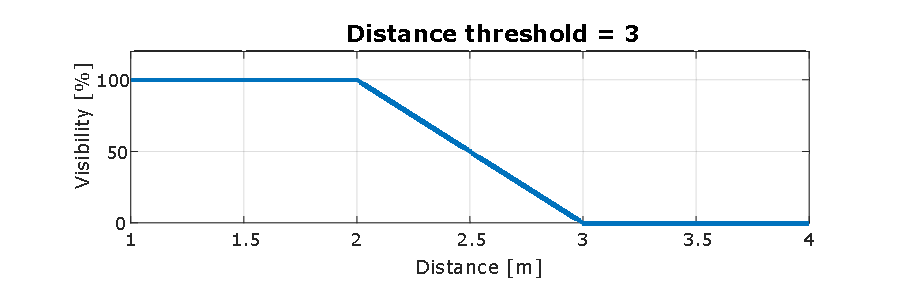
\includegraphics[width=\textwidth]{img/falloff.eps}
        \caption{Falloff}
        \label{fig:falloff}
    \end{figure}
    
    Finally, the threshold.py script outputs a bag file named \\ \textttt{<dataset>\_<threshold>\_tags.bag}, which is then sent to the estimator that outputs the pose estimates in low visibility into a bag file named \texttt{<dataset>\_<threshold>\_est.bag}.
    
    \subsection{Adding noise}
    \label{sec:noise}
    The second simulation assumes that there are floating particles in the water that bring noise into tag corner detection. We simulate this by corrupting the tag corner detections by random noise of a given variance. We are using the fact that the EKF in RCARS uses the tag corner detections as observations rather than the tag pose obtained by OpenCV. As a result of this holistic approach, we can improve the tracking by changing the PixelStd parameter in the EKFSettings.info file. The PixelStd parameter represents the pixel variance (the squared pixel standard deviation) of the tag corner detections.
    
    In full visibility, we use a pixel variance of 25 pixels. After adding noise to the corners, we raise this variance accordingly. For example, for noise with variance of 100 pixels, we set the \textit{PixelStd} parameter to 125.
    
    The workflow is similar to the thresholding. First, we obtain the \textttt{<dataset>\_tags.bag} file with full visibility from the detector. Second, the \textttt{add\_noise.py} script adds random noise with Gaussian distribution with zero mean and a given standard deviation. It uses the pseudo-random number generators Python module random\footnote{\url{https://docs.python.org/2/library/random.html}} with a seed 250. Finally, a file named \\ \textttt{<dataset>\_<standard\_deviation>px\_<PixelStd\_parameter\_value>\_tags.bag} is output, which is then processed by the estimator to obtain the pose estimates in the file \\
    \textttt{<dataset>\_<standard\_deviation>px\_<PixelStd\_parameter\_value>\_est.bag}.



\section{Evaluation method}
\label{sec:evaluation}
We evaluate the accuracy of the RCARS pose estimation by computing the Euclidean distance between the 3D position of the smartphone estimated by RCARS and the position measured by the motion capture (mocap). 
This section describes the evaluation method used in this thesis.
 
For data analysis and plotting, we use MATLAB. Thus, we wrote several MATLAB scripts to load the CSV files containing the pose estimates.
 
The filter and the mocap are two independent systems that do not communicate with each other. To be able to compare them, their coordinate frames have to be aligned and their samples synchronized. When this is not done correctly, it leads to bias in error calculations.


    \subsection{Coordinate frames}
    \label{sec:coords}
    For alignment, the goal is to find a common coordinate frame for RCARS and the mocap. There are several coordinate frames used in these systems:
    
    \missingfigure[figwidth=\textwidth]{Coordinate frames}
    \begin{itemize}
        \item Mocap
        \begin{itemize}
            \item world\_mocap: The laboratory.
            \item tag\_mocap: The tag rigid body, will serve as a reference frame.
            \item phone\_mocap: The phone rig.
        \end{itemize}
        \item RCARS
        \begin{itemize}
            \item world\_RCARS: This frame is initialized when RCARS starts receiving messages.
            \item tag\_RCARS: The frame of the reference tag.
            \item camera\_RCARS: This frame is used by the detector, which determines the immediate pose of the tag; as well as the estimator, which instead of using the pose from the detector it uses the corner locations in pixel coordinates that are transformed into this frame and the filter further estimates their pose here.
            \item IMU\_RCARS: The IMU measures in this frame.
        \end{itemize}
    \end{itemize}
    
    In our method, we select a reference tag as the common coordinate frame. In the case of the mocap, we create a rigid body for this tag and transform the smartphone pose measurements into the local coordinate frame of the marker as follows:
    \begin{equation}
        \label{eq:mocapTransform}
        phone_{mocap}^W * (tag_{mocap}^W)^{-1} = phone_{mocap}^{T} 
    \end{equation}
    \todo{Indexes}

    This process is similar for RCARS, where we start recording the dataset with the camera pointing at the reference tag and then use it to transform all pose estimates from the RCARS global frame into the local frame of the tag:

    \begin{equation}
        phone_{RCARS}^W * (tag_{RCARS}^W)^{-1} = phone_{RCARS}^{T}
    \end{equation}

    For also aligning the orientation, the marker has to be placed in the laboratory in a way that its mocap rigid body axes are the same as the RCARS tag axes to ensure pitch, yaw, and roll consistency. Provided proper marker placement, the orientation can be aligned by including the rotation matrix of the tag in the transformation matrix in \autoref{eq:mocapTransform}.

\section{Time synchronization}
    \label{sec:time_sync}
    After the poses from RCARS and mocap are aligned into a common coordinate frame, they have to be synchronized based on time. 
 
    It is assumed that the mocap dataset is always longer than the phone recording because, in our experiments, the recording on the mocap controller computer is started by the same person as the smartphone recording. Therefore, there is always a few second delay while the person moves to the initial position and starts recording on the smartphone. This is shown in Fig.X, where the recording on the smartphone was started 11 seconds after the mocap.
    
    \missingfigure[figwidth=\textwidth]{Delayed position}
    
    Since there is no grouping element in the CSV files of mocap and RCARS, we compute the cross-correlation between the positions in a given axis to find the count of samples that the mocap is ahead of RCARS. The choice of the axis depends on the range of motion in the dataset. From our tests, we prefer to use the x- or y-axis, since they are usually better estimated than the z-axis representing the height.

    Also, we found that the region for cross-correlation computing should not be the whole dataset but only the first few seconds. This is because we start the dataset recording with the camera pointing at the reference tag; therefore, even in the case when the filter is diverging, the error should be zero at the beginning and increase over time. Another case when taking only the beginning of the dataset is necessary is shown in Fig.X, where a gradually increasing delay in the dataset causes the cross-correlation to be maximum for the alignment of the second half of the dataset as a global optimum. By computing the cross-correlation only from the beginning of the dataset, we ensure that we find the initial alignment, not a global optimum.

    \missingfigure[figwidth=10cm]{Increasing delay}

\section{Error computation}
\label{sec:error}
    When the positions are aligned and synchronized, the error can be finally obtained by computing the Euclidean distance between them as follows:
    
    \begin{equation}
        error = \sqrt{(mocap.x - RCARS.x)^2 + (mocap.y - RCARS.y)^2 + (mocap.z - RCARS.z)^2}
    \end{equation}

    The result is demonstrated on an example dataset in Fig.X, where the estimated pose is diverging from the ground truth, causing an increasing error over time.
    
    \missingfigure[figwidth=10cm]{Error per frame}
    
    To evaluate the decreased visibility effects on the pose estimation, we run the estimator on many different thresholds and noise-corrupted detections, as shown in Fig.X. These estimates are then joined in one plot showing the mean error per sample for a given threshold or noise standard deviation.

\chapter{Experiment}
\section{Setup}
Calibration and bias free comparison is essential for our experiment. This section describes the specific setup and conditions that our experiments were performed in.

    \subsection{Laboratory}
    The experiments took place at the Human-Computer Interaction laboratory\footnote{\url{http://hci.fi.muni.cz/}} at the Faculty of Informatics, Masaryk University in Brno. As shown in Fig. \ref{fig:hcil}, the markers were randomly placed across the room, covering an area of 5.4 x 6.6 meters; with the markers attached both on horizontal and vertical surfaces.
    
    \begin{figure}
        \includegraphics[width=8cm]{example-image}
        \caption{HCIL}
        \label{fig:hcil}
    \end{figure}
    
    The laboratory is equipped with a high-quality motion capture system from Optitrack\footnote{\url{https://optitrack.com/products/prime-13w/}} that uses 16 ultra-wide cameras (Prime13W), offering high-precision and low-latency tracking with up to 240 FPS capture rate. Tracking of an object is realized by spherical retroreflective markers detected by the cameras. This system is controlled by Motive software, which provides calibration, creating rigid bodies, and recording.
    
    Before recording the datasets, a new calibration was performed following the documentation\footnote{\url{https://v20.wiki.optitrack.com/index.php?title=Calibration}}, with exceptional results with the mean 3D error of 0.673 mm. In our experiments, the average error per marker was 0.1mm for the static marker, and 0.4mm for the moving smartphone.

    \subsection{Markers}
    To find the pixel standard deviation of the marker detections in the conditions of our experiment, we built a static scene with the phone recording two markers at the distances of 1 m and 3 m for one minute. We calculated the average standard deviation of the detected corners, resulting in 0.40811 pixels for the marker at 1 m and 0.44091 pixels for the marker at 3 m. 
    
    The default PxStd parameter value for RCARS is 25 pixels. However, since we are recording in a higher resolution, we rather do not decrease this value and leave it on default.
    
    \begin{itemize}
        \item apriltags
        \item in EKFsettings.info, number of dynamic tags is set to 30. I used 27 AprilTags downloaded from here: \url{https://robot2016.mit.edu/sites/default/files/documents/project_apriltag36h11.pdf}
        \item placed on flat surfaces or attached with pritt gum, or just loosely on a chair, being careful not to bend them
    \end{itemize}
    
    \subsection{Phone}
    The smartphone we used is the OnePlus 6 running on Android 9 and equipped with a 16 MP, f/1.7, wide-angle camera (25mm (wide), 1/2.6") and the BMI160\footnote{\url{https://www.bosch-sensortec.com/bst/products/all_products/bmi160}} IMU manufactured by Bosch Sensortec\footnote{\url{https://www.bosch-sensortec.com/}}.
    
    \subsection{Intrinsic calibration}
    The intrinsic camera calibration was performed in the laboratory to assert equal lighting conditions than in the datasets recordings. We used the OpenCV algorithm\footnote{\url{https://docs.opencv.org/2.4/modules/calib3d/doc/camera_calibration_and_3d_reconstruction.html}} that calculates both the camera matrix and the radial and tangential distortion coefficients from a chessboard pattern. 
    We used a chessboard pattern with the count of inner corners along both sides of 9 x 6 and printed it on an A4 paper. The dimensions of one chessboard square were 25 x 25mm. The pattern, as well as the calibration images and coefficients, are provided in the attachments. 
    The calibration images were following the Matlab camera calibration workflow\footnote{\url{https://www.mathworks.com/help/vision/ug/single-camera-calibrator-app.html}}. As it says, to achieve a good camera calibration, between 10 and 20 images of the checkerboard pattern should be used. In addition, the images should be captured at a distance roughly equal to the distance from the camera to the objects of interest, without using autofocus or changing the zoom settings between images. Furthermore, since lens distortion increases radially from the center of the image and sometimes is not uniform across the image frame, the images should be taken at different orientations relative to the camera and the pattern must appear close to the edges of the captured images.

    \subsection{Extrinsic calibration}
    Due to the extrinsic calibration, we have to know where the IMU is located in the device. We tried to figure out this location from the OnePlus 6 motherboard photos. Although it indicated possible locations, the exact one was not clear. 
    Therefore, we used the online extrinsic calibration provided by RCARS. The calibration process, described in chapter X, returned the relative transformation estimate depicted in Fig. \ref{fig:extrinsic}. 

    \begin{figure}
        \includegraphics[width=8cm]{example-image}
        \caption{Extrinsic calibration - IMU 50cm in front of the camera}
        \label{fig:extrinsic}
    \end{figure}
    
    However, note that this estimate is still an approximation and may not reflect the true IMU location, thus the results may be affected by this error.
    
    \subsection{Phone rig}
    To track the phone pose with the motion capture system, we mount retroreflective markers tracked by the cameras on the phone. Thus, we built a custom rig from skewers and rubber bands, shown in FigX. Following the marker placement recommendations from the documentation\footnote{\url{https://v20.wiki.optitrack.com/index.php?title=Rigid_Body_Tracking}}, we attach five spherical markers on the skewer edges asymmetrically, to avoid congruency. 
    When a rigid body of this rig is created in Motive, its pivot point is at its geometric center. Thus, to put the pivot point to camera location, we measure the distance of the camera lens from the geometric center and translate the pivot point in Motive accordingly.
    
    \begin{figure}
        \includegraphics[width=8cm]{example-image}
        \caption{Phone rig}
        \label{fig:rig}
    \end{figure}

    This phone rig proved to be robust enough against deflection and, with the proper holding of the device, the rig is trackable by the motion capture system throughout the whole dataset with minimal detection losses.
    
    \subsection{Motion capture to filter estimation}
    As proposed in chapterX, the poses have to be aligned according to a common origin to be able to compare the poses measured by the motion capture and the filter. In this case, the origin is set to be the AprilTag with id 1.
    
    For position, we tackle the alignment as follows. The tag frame origin of the detected tag in OpenCV is in its geometrical center. Also, when a rigid body is created in Motive, its pivot point is placed at its geometric center. Thus, for tracking of the tag with motion capture, the reflective markers are placed onto the four corners of the tag, and a rigid body is created consequently. This way, we ensure that the origin of the marker pose is the same for both RCARS and motion capture.
    
    To be able also to compare the orientation of the mocap and the filter, we take the orientation in the filter as a reference. When OpenCV detects the tag, the tag is assigned orientation axes as shown in Fig.X. The axes of the camera are aligned with the tag when the phone is laying flat on the tag with the camera on top. Thus, initializing the axes for the tag and the phone in the same way, allows us to also compare the orientation of the mocap measurements and the filter estimates.T
    
    \begin{figure}
        \includegraphics[width=8cm]{example-image}
        \caption{Axes}
        \label{fig:axes}
    \end{figure}

    Since a new rigid body in motive has its axes aligned with the global coordinate axis, we place the tag aligned with the global frame. Then we lay the phone on the tag so that their geometrical centers overlap, as shown in FigX. Now the new rigid bodies for the tag and the phone can be created.
    
    \subsection{Recording}
    For recording the datasets on the smartphone, we used iMareCameraRecorder, developed by Jan Čejka. A recording contains accelerometer, gyroscope, and magnetometer measurements, and camera images with their corresponding timestamps. Note that the camera frames and the IMU samples are not synchronized as in the case of the specialized VI-Sensor, which may negatively affect the performance of the estimator.
    
    The application contains a configuration file for setting the image resolution and sampling rates. In the experiments, we used 1280x720 resolution, 30 frames per second, and the IMU sampling frequencies of 200Hz for gyroscope and 400Hz for the accelerometer. However, due to RCARS input requirements, we downsample the accelerometer to match the gyroscope frequency.

	
	\subsection{Computer}
	For running RCARS for estimation and MATLAB for evaluation, we primarily use the Lenovo Z580 laptop with Intel Core i7-3612QM 2.10GHz CPU and 8 GB of RAM.  In addition, for faster processing, we use a PC in the HCI laboratory with Intel(R) Core(TM) i7-8700 3.20GHz CPU and 32 GB of RAM.
	
	\subsection{RCARS}
	To run RCARS, we downloaded a Ubuntu 14.04 LTS virtual machine accessible on Nootrix.com\footnote{\url{https://nootrix.com/diy-tutos/ros-indigo-virtual-machine/}}, which has already preinstalled ROS Indigo and ROS tools. We tried to run it on the newest Ubuntu 18.04 first, however, we had dependency issues and failed to do so, similarly to other users discussing on Bitbucket\footnote{\url{https://bitbucket.org/adrlab/rcars/issues/4/rcars_detector_node-cant-run}}. 
    On this virtual machine, we installed RCARS according to the instructions in the project's repository\footnote{\url{https://bitbucket.org/adrlab/rcars/wiki/Home}}.
	Since we are recording our datasets in HD resolution, working with a large amount of markers, and running RCARS on a virtual machine, we run the detector first, save the detection results, and then run the estimator separately. Moreover, we play all bag files in slower speed to lower the computational demands and ensure the best detection and estimation possible.

\section{Datasets}
As discussed in \autoref{sec:simulating}, the underwater conditions are simulated in two ways: by discarding the detected tags according to their distance from the camera, and by adding noise to the detected tag corners.
 
Each simulation is executed on three different datasets: \textit{1CW}, \textit{2CCW}, and \textit{3RAND}. Figures \ref{fig:dataset06}, \ref{fig:dataset07}, and \ref{fig:dataset08} show the 2D and 3D trajectories of both the filter estimation and the mocap measurements, as well as the error per frame for each dataset. All of these datasets are available in the attachments of this thesis, including the bag files with the recordings, the motion capture CSV files, and the estimated CSV files. Note that we were not always working with the full lengths of the datasets; therefore, the intervals are provided in the parameter file for each dataset.

\todo[inline]{Show all datasets? If yes, which plots?}

In datasets \textit{1CW} and \textit{2CCW}, we walk slowly one time around the room clockwise and counter-clockwise, respectively, avoiding rapid changes in movement or orientation; nevertheless, shake still occurs in the image due to walking. 

Dataset \textit{3RAND} contains random trajectory movement with several fast motions to test both the filter robustness and outlier recovery. This kind of incautions use occurs when the system is used by inexperienced users, not aware of the importance of minimizing motion blur and shake.

The error per frame for \textit{1CW} is 13~cm, for \textit{2CCW} is 22~cm, and for \textit{3RAND} is 32~cm. The way the error occurs in the datasets differs; for example, while the error in \textit{2CCW} accumulates throughout the whole dataset, the error in \textit{3RAND} jumps at a certain point due to a fast movement, but then starts converging to its true position, which is again disrupted by the subsequent outliers.

\begin{figure}
    \includegraphics[width=\textwidth]{img/Dataset06.png}
    \caption{Dataset \textit{1CW}. Top-left: 3D visualization of the trajectory. Top-right: Difference between estimated and ground truth position per frame. Bottom: Estimated and ground truth position per axis.}
    \label{fig:dataset06}
\end{figure}

\begin{figure}
    \includegraphics[width=\textwidth]{img/Dataset07.png}
    \caption{Dataset \textit{2CCW}}
    \label{fig:dataset07}
\end{figure}

\begin{figure}
    \includegraphics[width=\textwidth]{img/Dataset08.png}
    \caption{Dataset \textit{3RAND}}
    \label{fig:dataset08}
\end{figure}


\section{Results}
    
    \subsection{Distance threshold}
    We estimated a number of thresholds in the interval from 1.5 to 5~m, focusing primarily on the thresholds below 3~m; thus, the thresholds are denser in the interval from 1.5 to 3~m, with an offset of 10~cm, while the more distant thresholds than 3 meters are estimated every 20~cm. This subsection gives commentary to the results.
    
    \subsubsection{Same errors, different plots}
    By decreasing the distance threshold, the count of detected images also decreases. When there is no image detected, the estimations are based only on the inertial measurements, and therefore the filter starts drifting away. This is shown in \autoref{fig:07_drift} for the dataset \textit{2CCW} --- even though the error at 1.8~m is lower than at 2.4~m by almost 5~cm, there is a significant difference in the estimation process, and thus also in the AR experience. While at 2.4~m the error accumulates gradually, at 1.8~m the filter starts diverging several times and jumps back near its true position when a marker is detected.
    
    \begin{figure}
        \includegraphics[width=\textwidth]{img/07_drift.png}
        \caption{Dataset \textit{2CCW} estimations at 2.3 m on the left, and 1.8 m on the right. Note that even though the mean error is lower at 1.8 m, the pose is drifting away in the highlighted areas; while the estimation at 2.3 m contains no drift.}
        \label{fig:07_drift}
    \end{figure}
    
    \subsubsection{Mean error per threshold}
    \autoref{fig:mean_error__per_threshold} shows the mean error per threshold for each dataset. Although we expected that with decreasing threshold, the error would gradually rise, the results do not fully follow this inverse proportionality.
    
    \begin{figure}
        \includegraphics[width=\textwidth]{img/thresholds.png}
        \caption{TODO: Horizontally. Mean error per threshold plots for each dataset.}
        \label{fig:mean_error__per_threshold}
    \end{figure}
    
    Instead, every dataset contains a threshold below 3~m where an outlier occurs, i.e., where the error significantly lower than the error in the neighboring thresholds. What is more, the errors of these outliers are at times as low or even lower than in 100~\% visibility, resulting in the peaks shown in FigX. For example, in the case of the dataset 1CW, where the mean error per sample at full visibility is 14~cm, but at 2.5~m is only 9~cm. For the dataset \textit{2CCW}, this occurs at the threshold of 2.2~m, with a 1~cm lower error than in the full visibility estimate.
    
    To verify that the peaks are not caused by the detector or estimator running too fast, we executed both the detection and estimation repeatedly on slower speeds and different computers. However, the results still stay the same.
    
    \subsubsection{Minimum threshold}
    With the threshold below 2~m, the estimation in all datasets often diverges by tens of meters. \autoref{fig:low_thresholds} contains plots showing the errors per frame in low thresholds for all datasets.
    
    \begin{figure}
        \includegraphics[width=\textwidth]{img/low_thresholds.png}
        \caption{Errors per frame in low thresholds}
        \label{fig:low_thresholds}
    \end{figure}
    
    We are interested in finding a minimum threshold where the tracking still reaches similar accuracy to the tracking in higher visibility. If the minimum threshold is taken from the mean error per threshold in \autoref{fig:mean_error__per_threshold}, \autoref{tab:edge_thresholds} shows the result, along with the average number of tags detected per frame in the estimation. The results indicate that at the visibility below 2.2 m, frequent marker detection losses occur, which causes the pose to diverge. This drift also happens when there is no marker detected in more than one image out of four.
    
    \begin{center}
        \begin{table}
            \begin{tabular}{l|lll}
                \toprule
                & 1CW & 2CCW & 3RAND \\
                \midrule
                Threshold (m) & 2.2 & 2.2 & 2.5 \\
                Average detected tags & 0.7864 & 0.7453 & 0.6071 \\
                \bottomrule
            \end{tabular}
            \caption{Edge distance thresholds for datasets}
            \label{tab:edge_thresholds}
        \end{table}
    \end{center}
    
    \subsubsection{Discussion}
	The results show that too many markers in the image, or detecting also distant markers when already closer ones are detected, does not improve the estimation accuracy. What is more, as in the case of dataset 3RAND shown in Fig.X, the distant markers can even decrease the accuracy. Thus, redundant distant markers may be discarded to reduce the map size of the estimation problem and lower the computational demands.
	
	Answering the question of why the spikes in \autoref{fig:mean_error__per_threshold}, is not in the scope of this thesis and is subject to future research. However, we assume that one of the reasons why the estimates in lower visibility are less accurate than in higher visibility is that the distant markers bring false information into the estimation.
	
	For example, we assume that the peak in \textit{3RAND} at 3.6~m occurred as follows. While for higher thresholds there were more distant markers that contributed to the tracking well, at 3.6~m they are not detected anymore, but there are still distant markers that may bring false information due to their placement or the device movement, which harms the estimation. By lowering the threshold to 3.4~m, these tags are discarded, thus, not bringing false information into the estimation. 
	
	We also assume that this interference by distant markers is occurring periodically in the rest of the dataset 3RAND, as well as in 1CW. We suppose that it could be controlled by adjusting the EKF parameters PixelStd and MahalanobisTh. The pixel standard deviation parameter sets the impact of tag detection on the estimation; increasing it would cause fewer outliers, but for the price of lower accuracy. On the other hand, lowering the Mahalanobis threshold would result in more frequent outliers; thus, the tag poses would be more frequently reset, and the system would have a higher chance of recovery. 
    
    \subsection{Added noise}
    We added zero-mean Gaussian noise to the tag corner detections with the standard deviations of 2, 5, 8, 10, 15, and 20 pixels, and respectively raised the \textttt{PxStd} parameter, representing the squared pixel standard deviation in the EKF estimation. Since the value of this parameter in full visibility is 25 pixels, after corrupting the detection results with the noise of standard deviation $\sigma$, the resulting value for the PxStd is $25 + \sigma^2$. \autoref{fig:noise} shows the output of this simulation in a mean error per noise standard deviation plot for every dataset.

    \begin{figure}
        \includegraphics[width=\textwidth]{img/noise.png}
        \caption{TODO: Horizontal pltos. Errors per noise standard deviation}
        \label{fig:noise}
    \end{figure}
    
    The results are similar for the datasets \textit{2CCW} and \textit{3RAND}. By adding noise of even 2~pixels, the mean error per sample rises from 22~cm to 65~cm in \textit{2CCW}, and from 31~cm to 65~cm in \textit{3RAND}. After continually increasing the amount of noise, the mean errors in \textit{3RAND} stay on 65~cm +- 1~cm to up to 15~pixels, while the mean errors in \textit{2CCW} stay on 65~cm +- 5~cm up to 10~pixels, and at 15~pixels, the error rises to 80~cm per sample. However, with the noise standard deviation of 20~pixels, the mean error significantly decreases in both datasets.
    
    In contrast, the mean errors in \textit{1CW} rise and drop randomly, ranging from 13~cm at full visibility up to 109~cm at 8~pixels.
    
    \subsubsection{Discussion}
    The datasets \textit{2CCW} and \textit{3RAND} confirm that by taking into account the pixel variance in the EKF estimation, the estimation accuracy is kept on the same level, or may even increase due to the large variance parameter. 
 
    A subject of future work can be determining the PxStd value for the device, as we left it on the default 25~pixels, but it has a considerable influence on the estimation accuracy.
    
    
\chapter{Conclusion}
In this thesis, we analyzed the underwater challenges of AR systems that are based on hybrid pose tracking and use Kalman filters for sensor fusion. We first chose a solution that meets our requirements, RCARS, and utilized it for the use with smartphone recordings. Using this system, we evaluated the effect of decreased visibility conditions simulated in a laboratory equipped with a motion capture system as ground truth.

We simulated the underwater conditions by discarding markers according to their distance from the camera and by corrupting the detected corners by adding artificial noise to simulate water turbidity. 

The results on our datasets show that the pose estimation accuracy of the system in 2.2m visibility is on the same level as in 3, 4, or even 5m visibility. Thus, we conclude that the system does not need a high amount of markers to produce accurate pose estimates. Instead, the number of detected markers can be even decreased to reduce computational complexity and, thus, improve the estimation speed.

From our experiments, we learned that for EKF-based systems, proper configuration is critical for satisfactory pose estimation. The experiment of adding noise to the detection showed that when the correct pixel standard deviation parameter is provided, the system can produce precise pose estimates even in a very turbid environment. However, these parameters are device dependent; finding them is not trivial and requires some experience. 

\section{Future work}
Since even a low number of markers is enough for quality estimates, future work could concentrate on analyzing datasets with sparsely placed markers. For this purpose, the RCARS visualization package is helpful, because it provides live pose estimation in a 3D workspace and an image preview that contains both the marker detections and the corresponding estimations. This tool can also be used for finding the appropriate EKF parameters for the device to minimize the bias caused by improper EKF configuration. 

Furthermore, other devices could be used for testing, since the system is also affected by the field of view, the autofocusing system of the camera, and the camera and IMU synchronization.
The intrinsic camera calibration depends on the field of view, which depends on the focusing distance. Thus, the calibration parameters can be obtained only for one focusing distance. However, when the camera's autofocus is enabled, the focusing distance changes throughout the dataset, causing the calibration parameters to be outdated. This problem can be tackled by saving the calibration parameters for various focusing distances and interchanging between them online during the detection.
In the video recordings of our datasets, \textit{focus breathing} of the autofocusing system occurred, which brings the tags temporarily out of focus, leading to detection loss. The “focus breathing” can be solved either by using a smartphone with a better autofocusing system or by disabling the autofocus and setting the focus to a proper distance. However, due to poor lighting conditions underwater, the cameras use large apertures leading to a shallower depth of field in the image, which increases the amount of blur in the background and the foreground; thus, possibly harming detection.
 
Another possible source of bias in our experiment is the pose alignment between RCARS and the motion capture system. Thus, instead of using the absolute alignment into one coordinate frame, one could compare their relative measures, such as the angular velocity or the total distance covered.
 
The future work could also concentrate on the development of marker-less SLAM based solutions that detect natural features instead of markers. However, this may lead to higher computational demands on the mobile device in both the detection and the estimation. Moreover, simulating underwater conditions for such systems is a whole new challenge.


\printbibliography[heading=bibintoc] %% Print the bibliography.
\end{document}